\section{Lighting and shading in the scene}
\label{sec:shading}
\begin{figure}[H]\centering
\begin{minipage}{0.49\linewidth}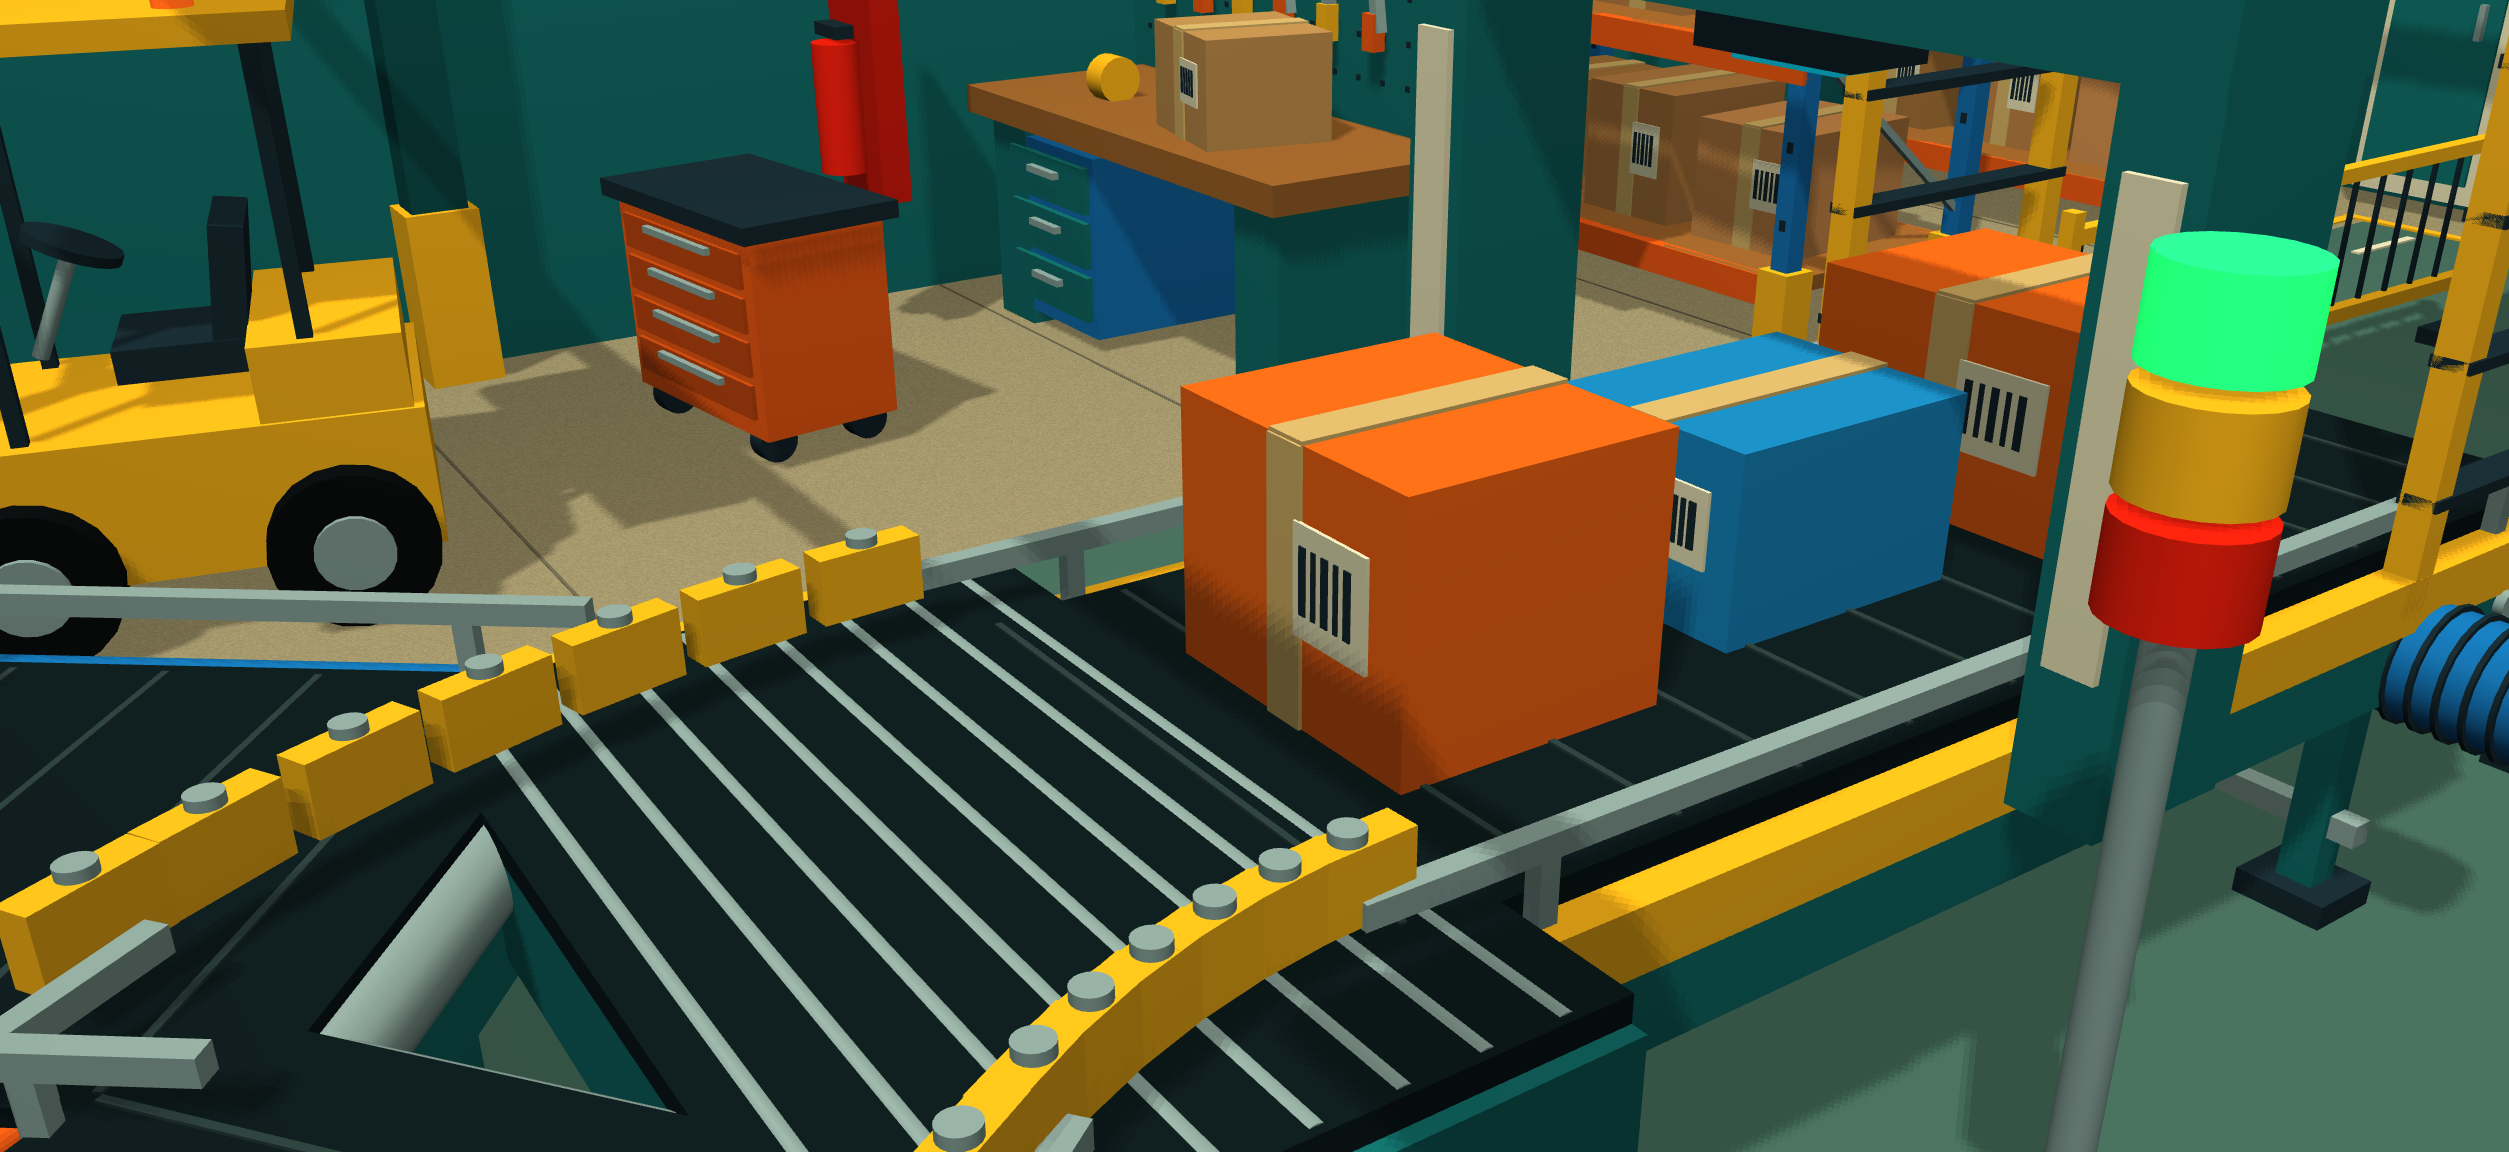
\includegraphics[width=\linewidth]{assets/phong_detail_crop.png}\par\small\textbf{A. Phong shading:} lighting calculated at each fragment.\end{minipage}\hfill
\begin{minipage}{0.49\linewidth}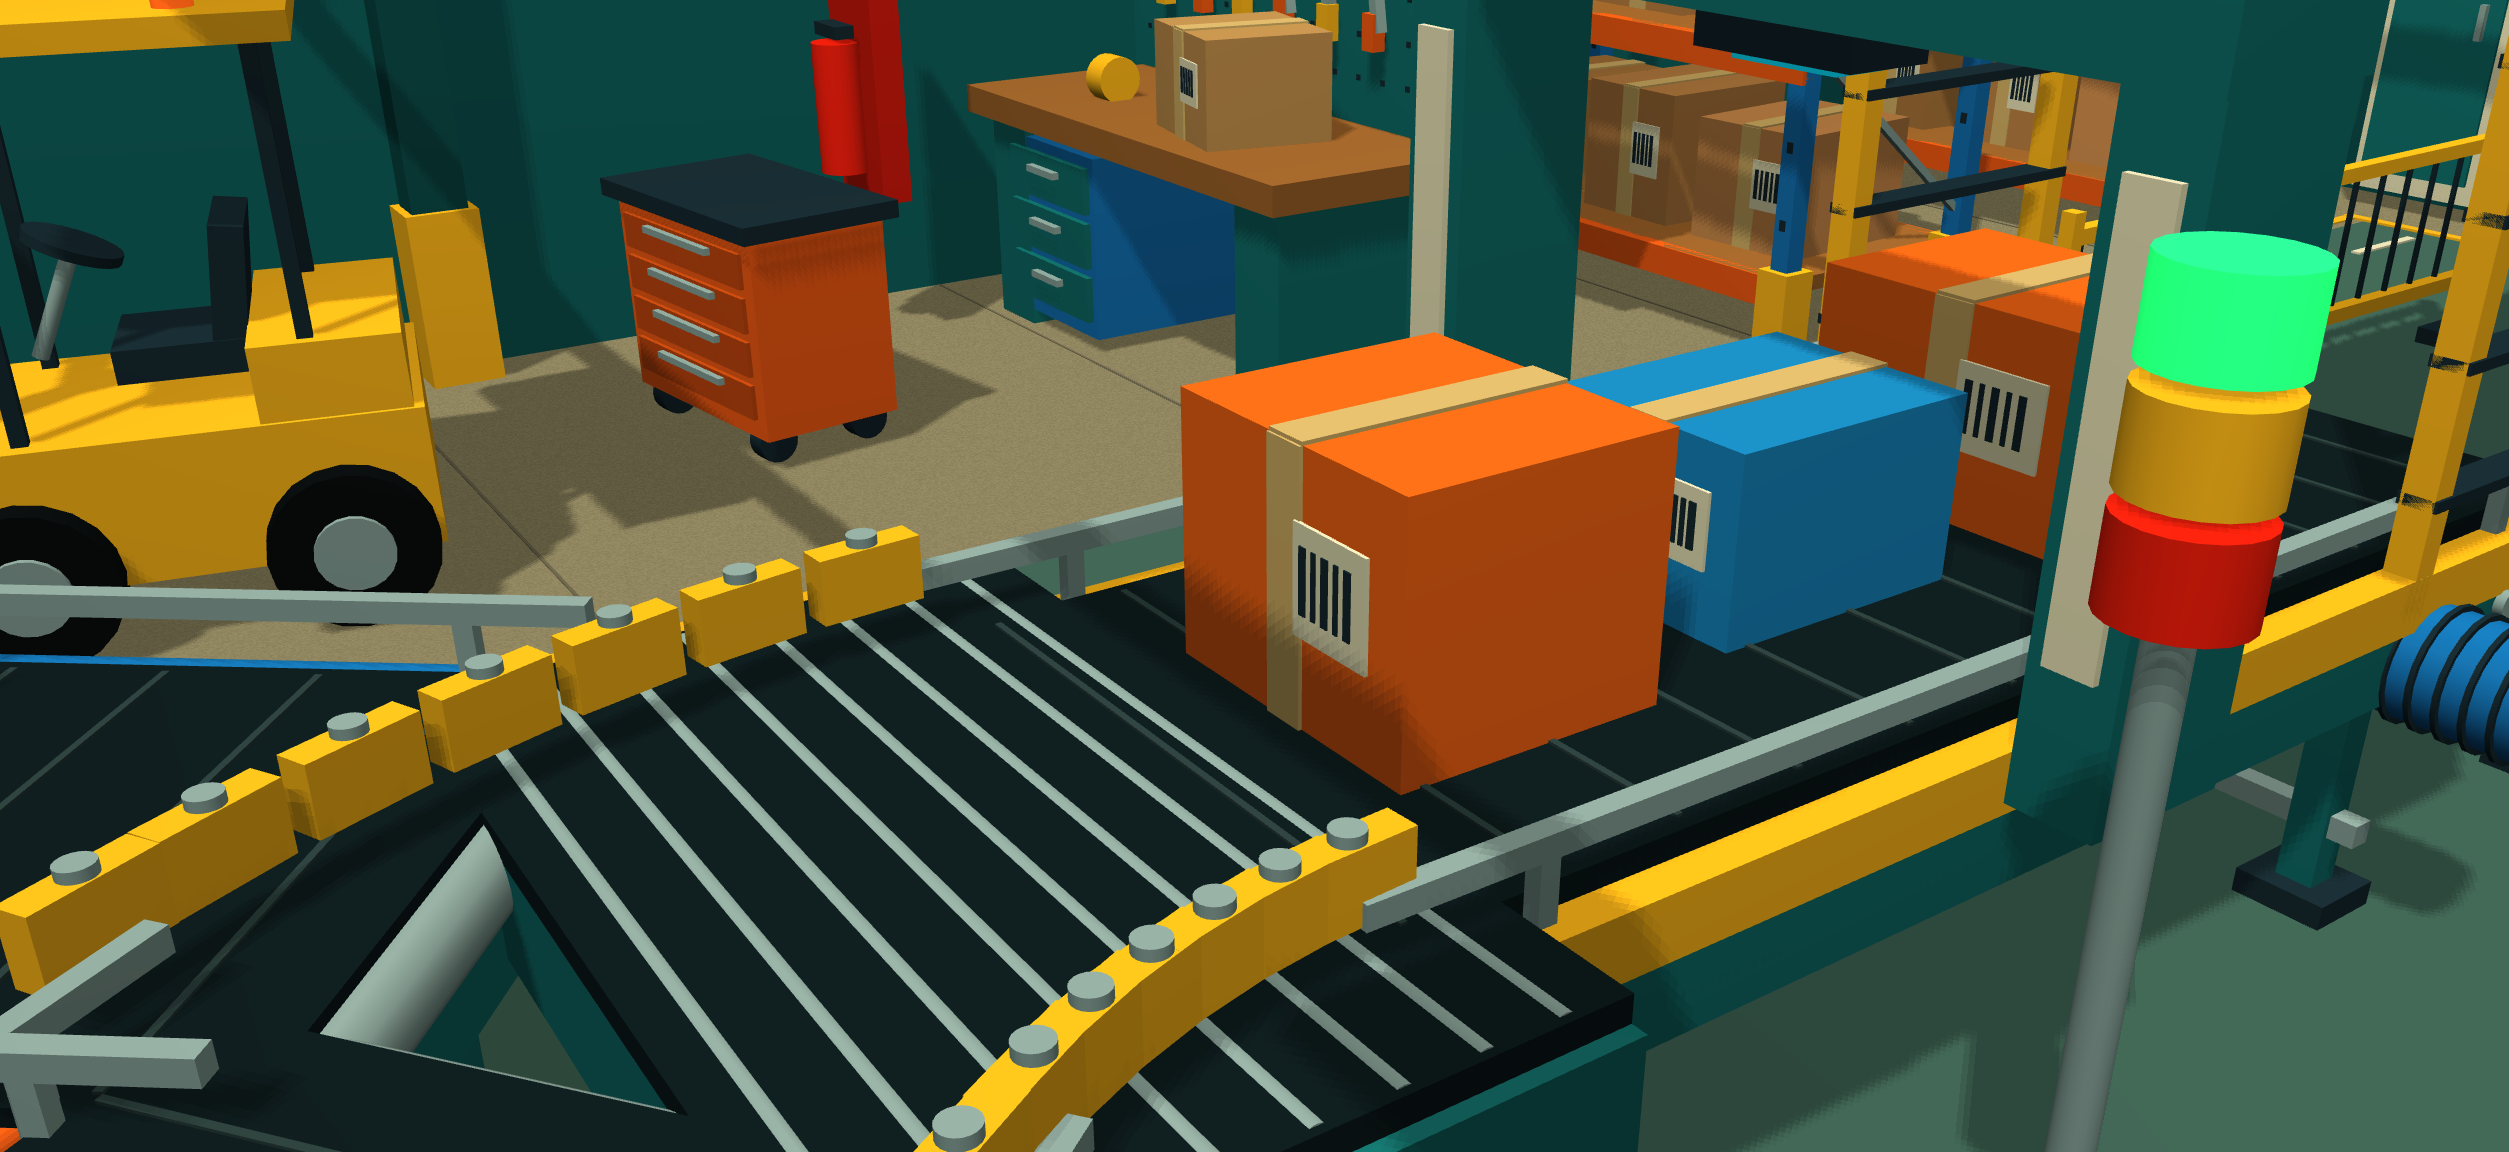
\includegraphics[width=\linewidth]{assets/gouraud_detail_crop.png}\par\small\textbf{B. Gouraud shading:} lighting calculated at vertices.\end{minipage}
\caption{Comparison at the same camera position and 24 s simulation time. Differences are most visible on the silver guides, rails and cylindrical roller; matte boxes show less variation.}
\end{figure}
\begin{shot}[0.85\linewidth]{assets/phong_detail_crop.png}{Detailed view of the default shading mode. Rail highlights and variations in face brightness provide depth cues.}
\callout{0.42,0.24}{0.17,0.12}{Metal highlights}
\callout{0.58,0.52}{0.80,0.80}{Matte box face}
\end{shot}
\subsection{Implemented illumination model}
Let $B$ be base RGB color, $C$ light color, $N$ the unit normal, $L$ the direction toward light, and $V$ the direction toward the camera. A dot product measures how closely directions align; RGB products act component by component.
\par{\small\begin{tabularx}{\textwidth}{@{}L{24mm}Y@{}}\toprule
\textbf{Term} & \textbf{Contribution and implemented equation}\\\midrule
Ambient & Provides background illumination. With $t=(N_y+1)/2$, $I_a=B[(1-t)(.20,.22,.21)+t(.48,.50,.47)]$.\\
Diffuse & Uses the Lambert cosine rule: $I_d=BC\max(N\cdot L,0)$.\\
Specular & Produces highlights. $H=\operatorname{normalize}(L+V)$; $u=\operatorname{clamp}((m-10)/70,0,1)$; $S=.22u^2(3-2u)\max(N\cdot H,0)^m$. Contribution is $SC$.\\\bottomrule
\end{tabularx}}\par
The default uses Phong shading with the Blinn-Phong specular term above. Parcels use shininess $m=8$ (no specular contribution); rollers use 90 and guides use 55. The key \code{P} switches to Gouraud shading. Shadows and emission are evaluated per fragment in both modes.

\subsection{Phong reflection and shading formulas}
For one light, the classic Phong reflection model is
\begin{equation}
I_{\mathrm{Phong}}=k_a I_A+k_d C\max(N\cdot L,0)
+k_s C\max(R\cdot V,0)^m,\qquad R=2(N\cdot L)N-L.
\end{equation}
Here $I_A$ is ambient illumination; $k_a$, $k_d$ and $k_s$ are ambient, diffuse and specular material coefficients; and $m$ is the shininess exponent. RGB multiplication is component-wise. The project uses $\max(N\cdot H,0)^m$ in place of $\max(R\cdot V,0)^m$ for its Blinn-Phong highlights.

Phong shading interpolates vertex normals and evaluates illumination at each fragment $p$:
\begin{equation}
N(p)=\operatorname{normalize}\!\left(\sum_{i=1}^{3}w_i(p)N_i\right),
\qquad I_P(p)=F\bigl(N(p),L(p),V(p)\bigr).
\end{equation}
The function $F$ denotes the illumination model, and $N_i$ are vertex normals. The interpolation weights $w_i(p)$ are corrected for perspective and satisfy $\sum_iw_i(p)=1$.

\subsection{Gouraud shading formula}
Gouraud shading evaluates illumination at the three vertices and interpolates the resulting colors:
\begin{equation}
I_i=F(N_i,L_i,V_i),\qquad
I_G(p)=\sum_{i=1}^{3}w_i(p)I_i.
\end{equation}
Both modes use the same implemented illumination model. Gouraud shading may miss a small highlight inside a triangle when it is absent at all three vertices.
\source{\code{basic.frag}: \code{phong()}; \code{basic.vert}: \code{lightingAtVertex()}.}
